\documentclass[12pt, letterpaper]{article}
\usepackage{amsmath, amssymb, graphicx, tikz, pgfplots}
\usepackage[margin = 1.5in]{geometry}
\graphicspath{ {/} }

\topmargin 0in
\headheight 0in

\setlength{\parindent}{0pt}

\begin{document}
\title{STAT 230 Course Notes}
\author{Muhammad Talha, taught by Diana K. Skrzydlo }
\date{Fall 2017}

\maketitle

\section{Chapter 1}
There are three definitions of probability.

\subsection{Classical}
If you have a bunch of possible outcomes that are \emph{equally} likely, then the probability
of an event is:

\[
 p = \frac{\text{total \# of ways that event can occur}}{\text{total \# of outcomes}}
\] \\

E.g. Find the probability of rolling a 1 with a six sided die. 
\[
p = \frac{1}{6}
\]

\subsection{Relative Frequency}
If you have the ability to repeat an event under the same conditions, the probability of an
event is the proportion of time it occurs in infinite repetitions.

\subsection{Subjective}
The subjective probability of an event is how confident a person is that it will occur.

\newpage

\section{Chapter 2}
An experiment is a process that has multiple possible results and can be repeated.
For example, rolling a dice is an experiment. There are 6 possible results and it can be repeated.\\

A trial is one iteration of an experiment. For example, rolling one die.
An outcome is one of the possible results from one trial of an experiment.\\

A sample space is a set of all possible outcomes from one trial of an experiment.
For example, the sample space for rolling one die is \(\{1, 2, 3, 4, 5, 6\}\).\\

An event is a subset of a sample space.
For example, the event for rolling a 1 is \( \{1\} \subseteq \{1, 2, 3, 4, 5, 6\}\).
If an outcome is inside an event, then the event occurred. An event that contains 
one element is called simple, otherwise it is called compound.

\subsection{Probability of an event}
The probability of an event A is \(p\left(A\right)\) and it conforms to the following axioms:

\begin{itemize}
\item \(0 \leq p\left(A\right) \leq 1\)
\item \(\sum\limits_{a \in A} p\left(a\right) = 1\)
\end{itemize}

Notice that the probability of an event is the sum of the probabilities of its simple
events.\\

E.g. Let A be the event for rolling an odd number, A = \( \{2, 4, 6\} \).
\[
	p\left(A\right) = p\left(\{2\}\right) + p\left(\{4\}\right) + p\left(\{6\}\right) = \frac{1}{6} + \frac{1}{6} + \frac{1}{6} = \frac{1}{2}
\]

An easier alternative is using the definition of classical probability, which results in
the same answer.

\newpage

\section{Chapter 3}
\subsection{Counting Techniques}
Counting deals with the problem of counting how many ways there are to do something.
There are two major techniques that help with counting problems.

\subsection{Addition Rule}
Suppose we want to count the number of ways to do task 1 \emph{or} task 2. If task 1 can
be done in \(p\) ways and task 2 can be done with \(q\) ways, then the number of ways to
do task 1 \emph{or} task 2, provided they don't overlap, is \(p + q\).\\

E.g. Recall that a character is either a digit (0-9) or a letter (a-z). The number of possible characters are \( 10 + 26 = 36\).\\

Note that the addition rule can only be used in situations where the two tasks don't overlap, i.e. cannot happen at the same time. For example, counting the number of ways to roll 1 dice or roll 1 dice is \( \frac{1}{6} \), not \( \frac{2}{6} \).

\subsection{Multiplication Rule}
Suppose we want to count the number of ways to do task 1 \emph{and} task 2. The number of ways to
do this, provided they don't depend on each other, is \(p \times q\).\\

E.g. How many ways are there to flip a coin (H, T) and roll a dice (1-6)?
There are \(2 \times 6 = 12\) ways.\\

Note that the multiplication rule can only be used in situations where the two tasks don't depend on each other, i.e. whether or not task 1 occurs does not affect whether or not task 2 will occur. For example, the number of ways to flip a head and a tail (at the same time) is 0.

\subsection{Sampling}
Sampling means picking items from a set. There are two ways to sample items from a set: with or without replacement.\\

With replacement means its possible to get the same item twice. For example, its possible to flip a coin and get a head, and then flip a coin again to get another head.\\

Without replacement means its \emph{not} possible to get the same item twice. For example, if we draw a card from a deck of 52 cards we will never draw that same card (with same rank and suite) again.

\subsubsection{Sampling with replacement}
Suppose we have \(n\) items in a set and we want a sample of size \(k\). How many ways are there to do this?\\

We can think of this problem as a bunch of tasks where each task is picking one of the \(k\) items from the set. So then we have \(k\) tasks.\\

How many ways are there to do task 1 (picking first of \(k\) items)? 

\(n\)\\

How many ways are there to do task 2 (picking second of \(k\) items)? 

Note that we are sampling \emph{with} replacement, so it is possible to get the same result twice.
That is, its possible to get the first item we picked in task 1. 

So there are \(n\) ways to do task 2.\\

In general, there are \(n\) ways to pick the \(ith\) item (\(1 \leq i \leq k \)).\\

\[
\underbrace{
\begin{tabular}{|c|c|c|c|c|}
	\hline n & n & n & ... & n \\ \hline
\end{tabular}
}_\text{k times}
\]\\

Now, we want the number of ways to do task 1 \emph{and} task 2 \emph{and} .. \emph{and} task \(k\).
By the multiplication rule, there are 

\begin{equation}
n^k
\end{equation}

ways to sample \(k\) items from a set containing \(n\) items with replacement.\\

E.g. Suppose 3 students go to either one of 4 schools and students can go to the same school. How many ways are there for these 3 students to go to school?

There are \(4^3\) ways.

\subsubsection{Sampling without replacement}
Suppose we have \(n\) items in a set and we want a sample of size \(k\). How many ways are there to do this?\\

We can split the problem up into \(k\) tasks just like we did in the previous section. \\

How many ways are there to do task 1 (picking first of \(k\) items)? 

\(n\)\\

How many ways are there to do task 2 (picking second of \(k\) items)? 

Note that we are sampling \emph{without} replacement, so it is not possible to get the same result twice. That is, it is not possible to get the first item we picked in task 1. 

So there are \(n - 1\) ways to do task 2.\\

In general, there are \(n - (i - 1)\) ways to pick the \(ith\) item (\(1 \leq i \leq k \)).\\

\[
\underbrace{
\begin{tabular}{|c|c|c|c|c|}
	\hline n & n - 1 & n - 2 & ... & n - k + 1  \\ \hline
\end{tabular}
}_\text{k times}
\]\\

Now, we want the number of ways to do task 1 \emph{and} task 2 \emph{and} .. \emph{and} task \(k\).
By the multiplication rule, there are 

\begin{equation}
n(n-1)(n-2)...(n-k+1) = \frac{n!}{(n-k)!} = n^{(k)}
\end{equation}

ways to sample \(k\) items from a set containing \(n\) items without replacement. The abbreviated notation \(n^{(k)}\) is often referred to as \(n\) to \(k\) factors.\\

E.g. Suppose 3 students go to either one of 4 schools and students cannot go to the same school. How many ways are there for these 3 students to go to school?

There are \(4^{(3)}\) ways.\\

E.g. Suppose a PIN is a 4-digit number where each digit cannot be repeated. How many possible PINs are there?

There are \(10^{(4)}\) possible PINs.

\subsubsection{Examples of with/without replacement}
E.g. An IP address is 4 numbers, each between 0-255. How many possible IP addresses are there?\\

Note that an IP address can repeat numbers (E.g. 192.168.1.1) so we are sampling with replacement.
There are \(256^4\) possible IP addresses.\\

E.g. What is the probability a random IP address contains only odd numbers?\\

Let A be the event that contains all IP addresses that contain only odd numbers.

\[
	p\left(A\right) = \frac{|A|}{|S|} = \frac{128^4}{256^4} = \frac{1}{16}
\]\\

E.g. What is the probability a random IP address has at least one 0? \footnote{In general, if a problem contains the wording "at least", consider using the complement.} \\

We could try solving this problem by considering all possible sub cases, in which case we would need to deal with having one 0's, two 0's, three 0's, etc. Lets instead use the complement.

\[
	p\left(A\right) = 1 - p\left(\bar{A}\right) = 1 - p\left(\text{IP address contains no 0's}\right) = 1 - \frac{255^4}{256^4}
\]\\

E.g. What is the probability an IP address has all distinct numbers?

Note that if an IP address has all distinct numbers, that means numbers cannot be repeated. Therefore, we are sampling without replacement.

\[
	p\left(A\right) = \frac{256^{(4)}}{256^4}
\]\\

E.g. Suppose five people (A, B, C, D, E) apply to four jobs (1, 2, 3, 4). What is the probability A gets the job?

How many possible ways can the jobs be filled up? \(5^{(4)}\).

This can be solved with or without using the complement. \\

\begin{enumerate}
\item Lets first solve it without using the complement. Lets consider all the sub cases where A gets a job.

\begin{center}
\begin{tabular}{c c c c c}
A & \_ & \_ & \_ & \(4^{(3)}\) \\ 
\_ & A & \_ & \_ & \(4^{(3)}\) \\ 
\_ & \_ & A & \_ & \(4^{(3)}\) \\ 
\_ & \_ & \_ & A & \(4^{(3)}\) \\ 
\end{tabular}
\end{center}

There are 4 sub cases and the number of ways each sub case can happen is \(4^{(3)}\).
Therefore:

\[
	p\left(A\right) = \frac{4 \times 4^{(3)}}{5^{(4)}}
\]\\

\item Now, using the complement:

\[
p\left(\text{A gets a job}\right) = 1 - p\left(\text{A does not get a job}\right) = 1 - \frac{4^{(4)}}{5^{(4)}}
\]
\end{enumerate}

\subsection{Permutations}
A permutation is an ordering of \(k\) objects selected from \(n\) objects without replacement.\\

How many permutations are there? \(n^{(k)}\)\\

Note that a permutation \emph{is} a ordering. There is, order matters when dealing with a permutation.

\subsection{Combinations}
A combination is a subset of \(k\) objects selected from \(n\) objects without replacement.\\

Note that a combination \emph{is} a subset. That is, order does not matter when dealing with a combination. \\

How many combinations are there?

Lets first find out how many possibilities there are when order matters. \(n^{(k)}\)\\

Now, how can we get rid of the duplicates?\\

E.g. Consider the set \({1, 2, 3}\). How many ways can this set be rearranged?

\[
\{1, 2, 3\}, 
\{1, 3, 2\},
\{2, 1, 3\},
\{2, 3, 1\},
\{3, 1, 2\},
\{3, 2, 1\}
\]\\

We see there are 6, or \(3!\) ways to arrange three numbers. In general, there are \(k!\) ways to rearrange \(k\) objects. For each ordering of \(k\) objects in our permutation, we need to divide by the number of rearrangements of \(k\) objects in order to remove the duplicates.\\

There are

\begin{equation}
\frac{n^{(k)}}{k!} = \frac{n!}{k!(n-k)!} = {{n}\choose{k}}
\end{equation}

ways to select \(k\) objects from \(n\) objects without replacement and order doesn't matter.
The abbreviated notation \(n \choose k\) is often referred to as \(n\) choose \(k\).\\

There are several properties of \(n \choose k\) that you will study in MATH 239 but we will just discuss two of them.

\begin{enumerate}
\item 
\[
{n \choose k} = {n \choose n - k}
\]\\

This result can be proved using arithmetic but the logical proof is more interesting and easier to remember. The number of ways to include \(k\) objects is to equal to the number of ways to exclude \(n - k\) objects. After excluding \(n - k\) objects, we will be left with \(n\) objects.

\item
\[
{n \choose k} = {n - 1 \choose k - 1} + {n - 1 \choose k}
\]\\

Suppose one of the \(n\) objects is special. Then \({n \choose k}\) contains all the ways to choose \(k\) objects from \(n\) objects (whether or not we include the special object in our \(k\) objects). However, this should be equal to the number of ways to choose \(k\) objects including the special object plus the number of ways to choose \(k\) objects excluding the special object.\\

Note that the two sub cases don't overlap (cannot include and exclude the special object at the same time) so we can use the addition rule.
\end{enumerate}

E.g. Suppose you select 5 cards from a deck of 52 cards. Recall a standard deck of 52 cards has 4 suites and 13 ranks. What is the probability of getting a full house (3 cards of one rank and 2 cards of another rank)?\\

First, how many possible ways are there to select 5 cards out of 52 cards? \(52 \choose 5\)\\

We want 3 cards of one rank \emph{and} 2 cards of another rank. 

How many ways are there to select 3 cards of one rank? We need to select a rank: \(13 \choose 1\). Choosing a rank will get us 4 cards (one for each suite) \emph{and} we need to pick 3 cards of out these 4 cards: \(4 \choose 3\). Similarly, to get 2 cards of another (i.e. different) rank: \(12 \choose 1\) \emph{and} out of those 4 cards we need to pick 2: \(4 \choose 2\). So we get:

\[
\frac{{{13 \choose 1}{4 \choose 3}{12 \choose 1}{4 \choose 2}}}{{52 \choose 5}}
\]

\subsection{Arrangements with alike objects}

How many arrangements are there of the word: S T A T I S T I C S (10 letters, 3 S's, 3 T's, 1 A, 2 I's, 1 C)?

It is not \(10!\).\\

The problem is that there exists alike objects inside the word. For example, the letter S is repeated and two S letters cannot be distinguished between each other. As a result, there are no longer 10 possible choices for the first "slot". The first letter can now only be S, T, A, I, C (5 choices). How can we deal with this case?\\

What we can do is first treat all letters as distinct. Then there are \(10!\) ways to rearrange the word. Now, for each arrangement of the word, say:

\[
S_1 \, T_1 \, A_1 \, T_2 \, I_1 \, S_2 \, T_3 \, I_2 \, C_1 \, S_3
\]

there are multiple ways to rearrange that word so that it will look exactly the same:

\begin{center}
\(S_1 \,... S_2 \,... S_3\)\\
\(S_1 \,... S_3 \,... S_2\)\\
\(S_2 \,... S_1 \,... S_3\)\\
\(S_2 \,... S_3 \,... S_1\)\\
\(S_3 \,... S_1 \,... S_2\)\\
\(S_3 \,... S_2 \,... S_1\)\\
...\\
\(T_i \,... T_j \,... T_k\)\\
...\\
\(I_i \,... I_j\)\\
...\\
\end{center}

So in order to get rid of the over-counting we did by treating all letters as distinct, we need to divide by all possible ways to rearrange the alike objects. The number of ways to rearrange the S's inside the word is \(3!\), the number of ways to rearrange the T's inside the word is \(3!\) and similarly \(1!\), \(2!\), \(1!\) for A, I, C respectively.\\

So there are 

\[
\frac{10!}{3! \times 3! \times 1! \times 2! \times 1!}
\]

ways to rearrange the word S T A T I S T I C S.\\

In general, if you have \(n\) objects with \(n_1\) type 1's, \(n_2\) type 2's, ..., \(n_k\) type k's, there are:

\[
\frac{n!}{n_1! \times n_2! \times ... \times n_k!}
\]

ways to rearrange the \(n\) objects.

\newpage

\section{Chapter 4}
In this chapter we will formalize a lot of the concepts we learned in chapter 3, mathematically.

\subsection{Set theory for probability}
Recall that an event is a subset of a sample space. Therefore, all concepts from set theory learned in MATH 135 extends to events. Let A, B be events of a sample space.

\begin{gather*}
p\left(\text{A \emph{or} B occurs}\right) = p\left(A \cup B\right)\\
p\left(\text{A \emph{and} B occurs}\right) = p\left(A \cap B\right)\\
p\left(A\right) = 1 - p\left(\bar{A}\right)\\
p\left(\overline{{A \cup B}}\right) = p\left(\bar{A} \cap \bar{B}\right)\\
p\left(\overline{{A \cap B}}\right) = p\left(\bar{A} \cup \bar{B}\right)\\
p\left(A \cup B \right) = p\left(A\right) + p\left(B\right) - p\left(A \cap B\right)\\
p\left(A \cup B \cup C\right) = p\left(A\right) + p\left(B\right) + p\left(C\right) - p\left(A \cap B\right) - p\left(A \cap C\right)\\ - p\left(B \cap C\right) + p\left(A \cap B \cap C\right)\\
\end{gather*}

Note that \(p\left(A \cap B\right)\) is commonly abbreviated as \(p\left(AB\right)\).\\

Two events, A and B, are called mutually exclusive if \(AB = \emptyset\).

Two events are independent if \(p\left(AB\right) = p\left(A\right) p\left(B\right)\).

\subsubsection{Addition Rule Revised}
Recall that if task 1 can be done in \(p\) ways and task 2 can be done in \(q\) ways, then the number of ways to do task 1 \emph{or} task 2, assuming they don't overlap, is \(p + q\). Lets extend this concept to events. How many ways are there to do A \emph{or} B, that is, \(A \cup B\)? 
There are \(|A| + |B| - |AB|\) ways. However, if A and B don't overlap (i.e. cannot happen at the same time), then \(AB = \emptyset, |AB| = 0\). So there would only be \(|A| + |B|\) ways.\\

In general, we can only use the old addition rule when two events are mutually exclusive, that is, cannot happen at the same time. Otherwise, we need to subtract the number of ways the two events can happen at the same time.

\subsubsection{Multiplication Rule Revised}
Recall that if task 1 can be done in \(p\) ways and task 2 can be done in \(q\) ways, then the number of ways to do task 1 \emph{and} task 2, assuming they don't depend on each other, is \(p \times q\). Lets extend this concept to events. How many ways are there to do A \emph{and} B, that is, \(AB\)? There are \(|AB|\) ways. However, if A and B don't depend on each other, then \(AB = A \times B\footnote{\(A \times B\) is the cartesian product of A and B.}, |AB| = |A||B|\). So there would only be \(|A||B|\) ways.\\

In general, we can only use the old multiplication rule when two events are independent, that is, whether or not one event occurs does not increase/decrease the probability that the other event occurs.\\

Note that the reasoning for why \(AB = A \times B\) when events A and B don't depend on each other is tricky, and a bit unintuitive at first. Consider two events: A = flipping a coin and getting head, B = rolling a dice and getting an odd number. Clearly, \(A = \{H\}, B = \{2, 4, 6\}\). We know that flipping a head does not affect whether or not we get an odd number, so the total number of ways we can flip a head \emph{and} roll an odd number should just be all pairs of the two events, \((H, 2), (H, 4), (H, 6)\), that is, \(1 \times 3 = 3\) ways. In general, if two events are not independent, then we cannot do this and we need to apply another technique.

\subsubsection{Examples using revised rules}
E.g. Suppose we roll 2 dice. What is the probability that both dice rolls give an odd number?\\

We want \(p\left(\text{first dice is odd \emph{and} second dice is odd}\right)\). Are the two events independent? Whether or not we roll an odd number on the first dice should not increase/decrease the probability of rolling an odd number on the second dice. So they are independent and by the multiplication rule, the total number of ways are: \(\frac{3}{6} \times \frac{3}{6} = \frac{1}{4}\).\\

E.g. Let A = first dice rolls a 3. Let B = the sum of two dice rolls is 7. Are A and B independent?\\

In this case it is tricky to tell from intuition. We can try to figure out if \(p\left(AB\right) = p\left(A\right)p\left(B\right)\) and if it does, then A and B are independent. Clearly, \(p\left(A\right) = \frac{1}{6}\) and \(p\left(B\right) = \frac{|\{(1, 6), (2, 5), (3, 4), (4, 3), (5, 2), (6, 1)\}|}{6^2} = \frac{6}{6^2} = \frac{1}{6}\).

\(p\left(AB\right) = \frac{|\{(3, 4)\}|}{6^2} = \frac{1}{6^2}\).\\

Clearly, \(p\left(AB\right) = p\left(A\right)p\left(B\right)\) so A and B are independent.\\

E.g. Let A = first dice rolls a 3. Let C = the sum of two dice rolls is 8. Are A and C independent?\\

Lets try to figure out if \(p\left(AC\right) = p\left(A\right)p\left(C\right)\) and if it does, then A and C are independent.\\

\(p\left(A\right) = \frac{1}{6}\) and \(p\left(C\right) = \frac{|\{(2, 6), (3, 5), (4, 4), (5, 3), (6, 2)\}|}{6^2} = \frac{5}{6^2}\).

\(p\left(AC\right) = \frac{|\{(3, 5)\}|}{6^2} = \frac{1}{6^2}\).\\

We see that \(p\left(AC\right) \neq p\left(A\right)p\left(C\right)\) so A and C are dependent. How could we have arrived to the same conclusion by using intuition? It seems that whether or not the first dice roll is 3 increases/decreases the probability that the total is equal to 8. Suppose the first dice roll is not 3, and instead is 1. Then that makes C impossible since the highest possible total is 7. So then A and C are dependent.

\subsection{Conditional Probability}
The concept of conditional probability is related to dependence between two events. The probability of an event A, given another event B has happened is:

\begin{equation}
p\left(A|B\right) = \frac{p\left(AB\right)}{p\left(B\right)}
\end{equation}\\

Note that if A and B are independent, then this simplifies to \(p\left(A|B\right) = \frac{p\left(A\right)p\left(B\right)}{p\left(B\right)} = p\left(A\right)\). That is, whether or not B occurs does not affect the probability that A occurs. \\

Suppose that A and B are dependent. Why does the conditional probability of A given B divide by the probability of B? The reason why is because we limit the sample space to B. We are essentially asking the question: what is the probability of event A happening in all those cases where B happens.\\

E.g. Let A = first dice rolls a 3. Let C = the sum of two dice rolls is 8. What is \(p\left(A|C\right), p\left(C|A\right)?\)\\

Recall \(p\left(A\right) = \frac{1}{6}\), \(p\left(C\right) = \frac{5}{6^2}\) and \(p\left(AC\right) = \frac{1}{6^2}\) where A and C are dependent. Then:

\begin{gather*}
	p\left(A|C\right) = \frac{p\left(AC\right)}{p\left(C\right)} = \frac{\frac{1}{6^2}}{\frac{5}{6^2}} = \frac{1}{5}\\
	p\left(C|A\right) = \frac{p\left(CA\right)}{p\left(A\right)} = \frac{\frac{1}{6^2}}{\frac{1}{6}} = \frac{1}{6}\\
\end{gather*}

Notice that the probability of A increased from \(\frac{1}{6}\) to \(\frac{1}{5}\). The reason why is because if C occurs, that is, the total is 8, then the first dice roll could not have been a 1 (otherwise the total would be 7). There are only 5 possibilities the first dice roll could be, which is 1 less than the number of possibilities if the total was not 8. Therefore, A is more likely. Also, notice that C is more likely.\\

In general, dependence is a two way street. If A makes B more likely, then B makes A more likely. Similarly if A makes B less likely, then B makes A less likely.\\

E.g. Suppose we flip a coin 4 times. Let A = event where we get at least 3 heads. Let B = the event where the first flip is tails. What is \(p\left(A|B\right)\) and \(p\left(B|A\right)\)?\\

We could use the definition of conditional probability but instead we will solve this problem much more intuitively. This involves figuring out how many times A and B can occur together and dividing it by how many times B can occur.\\

How many ways can B occur? The first flip must be a tails and the other 3 flips can be head or tails. So there are \(2^3\) ways. 

Of those \(2^3\) cases, how many include event A? There is only one case that satisfies both A and B, \(\{T, H, H, H\}\). So \(p\left(A|B\right) = \frac{1}{2^3}\).\\

Similarly for \(p\left(B|A\right)\), how many ways can A occur? There are 2 sub cases: getting exactly 3 heads or getting exactly 4 heads. \(4 + 1 = 5\). Of those 5 cases, how many satisfy B? There is only 1, as mentioned above. So \(p\left(B|A\right) = \frac{1}{5}\).

\subsection{Product Rule}
Recall for two events A and B, the conditional probability of A given B is:
\(p\left(A|B\right) = \frac{p\left(AB\right)}{p\left(B\right)}\) and B given A is: \(p\left(B|A\right) = \frac{p\left(AB\right)}{p\left(A\right)}\). The product rule is just a rearrangement of conditional probability. The probability of A \emph{and} B is:

\begin{equation}
p\left(AB\right) = p\left(B\right)p\left(A|B\right) = p\left(A\right)p\left(B|A\right)
\end{equation}\\

Note that the product rule does make logical sense. The probability of A \emph{and} B is the probability that B occurs times the probability that A occurs given B has occurred, or the probability that A occurs times the probability that B occurs given A has occurred. This intuitive rule is also extendable:

\begin{gather*}
p\left(ABC\right) = p\left(A\right)p\left(B|A\right)p\left(C|AB\right)
\end{gather*}

\subsection{Partition Rule}
Suppose you have a sample space S that can be partitioned into a bunch of subsets that combine to make up S. That is, \(S = E_1 \cup E_2 ... \cup E_k\). Any event could have parts of \(E_i\) and so we can split it up into those parts.\\

\begin{center}
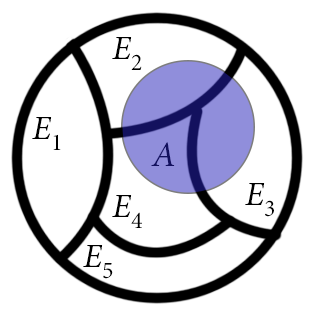
\includegraphics[width=3cm, height=3cm]{partition_rule}
\end{center}

Then for any event A: \(A = AE_1 \cup AE_2 ... \cup AE_k\). 

\begin{gather*}
p\left(A\right) = p\left(AE_1\right) + p\left(AE_2\right) + ... + p\left(AE_k\right) = \sum_{i = 1}^{k} \left(AE_i\right)
\end{gather*}

\begin{equation}
p\left(A\right) = \sum_{i = 1}^{k} p\left(E_i\right)p\left(A|E_i\right)
\end{equation}\\

Note that a often used partition of S is simply an event B and its complement \(\bar{B}\) since \(S = B \cup \bar{B}\).

\subsection{Bayes Rule}
Bayes rule is used to reverse the sign of conditional probability. For example, if we want to find \(p\left(A|B\right)\) but only have \(p\left(B|A\right)\), we can use bayes rule.

\begin{equation}
p(A|B) = \frac{p\left(AB\right)}{p\left(B\right)} = \frac{p\left(A\right)p\left(B|A\right)}{p\left(B\right)}
\end{equation}\\

\subsection{Example using all rules}
E.g Suppose 2\% of a population have a disease. A blood test for the disease gives a 5\% false positive rate and a 1\% false negative rate. What is the probability of a random person tests positive for the disease?\\

The first thing to note is that our sample space will contain the entire population of people. The second thing to note that is we have a partition of the sample space: all the people who have the disease and all the people who don't.\\

Let D = person has the disease. Let T = person tests positive for the disease. We know \(p\left(D\right) = 0.02, p(T|\bar{D}) = 0.05, p\left(\bar{T}|D\right) = 0.01\).\\

\(S = D \cup \bar{D}\). So by the partition rule and product rule:

\begin{align*}
p\left(T\right) &= p\left(D\right)p\left(T|D\right) + p\left(\bar{D}\right)p\left(T|\bar{D}\right)\\
&= 0.02(1 - 0.01) + 0.98(0.05) = 0.0688
\end{align*}

Suppose that someone tests positive. What is the probability they have the disease?\\

We want \(p\left(D|T\right)\). By Bayes rule:

\begin{align*}
p\left(D|T\right) &= \frac{p\left(D\right)p\left(T|D\right)}{p\left(T\right)}\\
&= \frac{0.02(1 - 0.01)}{0.0688}\\
&= 0.288
\end{align*}

\newpage

\section{Chapter 5}
We will now introduce the concept of random variables. As the name implies, random variables are random (i.e. they can take multiple values). The values that a random variable can take is called the range of the random variable.\\

Convention: X, Y, Z are often abbreviated as random variables and x, y, z are values they can take, respectively. Random variable is often abbreviated as r.v.\\

Random variables can be discrete or continuous. Discrete random variables are random variables who have a discrete range (finite or countably infinite). Continuous random variables are random variables who have a continuous range (uncountable infinite, like \(\mathbb{R}\)). For example a random variable that can take a value anywhere between 0 and 1.0 is continuous as there are uncountably infinite values in that range. This chapter will discuss discrete random variables.\\

The probability that X takes a value x is called the probability function of X:

\begin{equation}
f\left(x\right) = P\left(X = x\right) \;\;\; \forall x \in X
\end{equation}\\

The probability function of a random variable conforms to following axioms:

\begin{itemize}
\item \(0 \leq f\left(x\right) \leq 1\)
\item \(\sum\limits_{x \in X} f\left(x\right) = 1\)
\end{itemize}

The probability that X takes a value \(\leq\) x is called the cumulative distribution function of X:

\begin{equation}
F\left(x\right) = P\left(X \leq x\right) \;\;\; \forall x \in \mathbb{R}
\end{equation}\\

Note that cumulative distribution function is often abbreviated as c.d.f. Also note that it is defined for all real numbers.\\

The cumulative distribution function of a random variable conforms to following axioms:

\begin{itemize}
\item \(0 \leq F\left(x\right) \leq 1\)
\item \(\lim_{F\left(x\right)\to\infty} F\left(x\right) = 1\)
\item \(\lim_{F\left(x\right)\to{- \infty}} F\left(x\right) = 0\)
\item \(F\left(x\right)\) is non-decreasing
\end{itemize}

If \(x_o\) is the minimum then \(F\left(x_o\right) = f\left(x_o\right)\).

If \(x_o\) is the maximum then \(F\left(x_o\right) = 1\).

\(F\left(x\right)\) is non-decreasing because it is the sum of the values before it, that is, it is at least \(F\left(x - 1\right)\).\\

E.g. Graph the c.d.f for the following random variable X = number of 1's in 3 dice rolls:

\begin{center}
\begin{tabular}{|c|c|c|c|c|}
\hline
x & 0 & 1 & 2 & 3\\ \hline
\(f\left(x\right)\) & \(5^3/6^3\) & \(4\cdot(5^2)/6^3\) & \(15/6^3\) & \(1/6^3\)\\ 
\hline
\end{tabular}
\end{center}

\begin{gather*}
F\left(0\right) = P\left(X \leq 0\right) = f\left(0\right) = \frac{125}{216}\\
F\left(1\right) = P\left(X \leq 1\right) = f\left(0\right) + f\left(1\right) = \frac{5^3}{6^3} + \frac{4 \cdot 5^2}{6^3} = \frac{200}{216}\\
F\left(2\right) = P\left(X \leq 2\right) = f\left(0\right) + f\left(1\right) + f\left(2\right) = \frac{200}{216} + \frac{15}{6^3} = \frac{215}{216}\\
F\left(3\right) = P\left(X \leq 3\right) = 1
\end{gather*}
\begin{center}
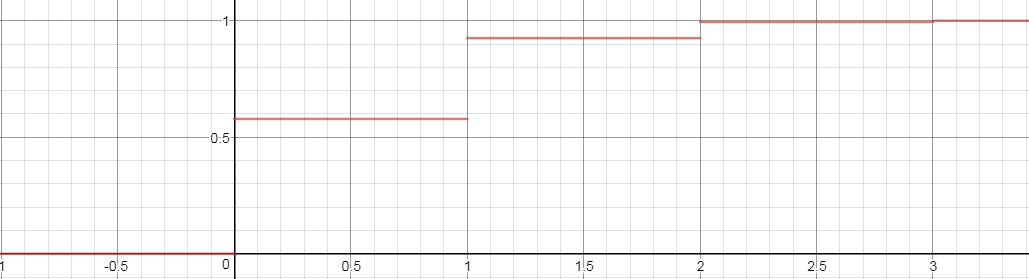
\includegraphics[width=15cm, height=5cm]{exampleF(x)}
\end{center}

So we see that \(F\left(x\right)\) is a right continuous step function with discontinuities at each value of x in X's range.\\

Also note that \(f\left(x\right) = F\left(x\right) - F\left(x - 1\right)\), that is, \(P\left(X = x\right) = P\left(X \leq x \right) - P\left(X \leq x - 1\right)\). 

\subsubsection{Discrete Uniform Random Variable}
Let X be a random variable that takes values in the range \(\{a, a + 1, ..., b\}\) such that each value is equally likely. Then we say X \emph{is a} discrete uniform random variable:

\begin{equation}
X \sim DU[a, b]
\end{equation}\\

E.g. Let X = value on die. Then \(X \sim DU[1, 6]\).\\

What is the probability function of X?

\begin{equation}
f\left(x\right) = P\left(X = x\right) = \frac{1}{b - a + 1}
\end{equation}\\

What is the cumulative distribution function of X?

\begin{equation}
F\left(x\right) = P\left(X \leq x\right) = 
	\begin{cases} 
      0 & x < a \\
      1 & x > b \\
      \sum\limits_{i = a}^{\left \lfloor{x}\right \rfloor} \frac{1}{b - a + 1} = \frac{\left \lfloor{x}\right \rfloor - a + 1}{b - a + 1} & a \leq x \leq b
	\end{cases}
\end{equation}\\

Note that, in the discrete uniform case, the cumulative distribution function has "jumps" of equal heights.

\subsubsection{Hypergeometric Random Variable}
Suppose you have \(N\) objects, \(r\) of which are successes and \(N - r\) are fails. Suppose we draw \(n\) objects without replacement and order doesn't matter. Let X be a random variable that counts the number of successes in those \(n\) objects. Then we say X \emph{is a} hypergeometric random variable:

\begin{equation}
X \sim Hyper(N, r, n)
\end{equation}\\

E.g. In lotto 6/49 six numbers are drawn from \(\{1, 2, ..., 49\}\) to be winning numbers. Players draw 6 numbers\footnote{"Draw" often implies without replacement and order doesn't matter.}. Let X = number of winning numbers a player draws. Then \(X \sim Hyper(49, 6, 6)\).\\

What is the probability function of X?

\begin{equation}
f\left(x\right) = p\left(\text{we draw $x$ successes \emph{and} $n - x$ failures}\right) = \frac{{r \choose x}{{N - r} \choose {n - x}}}{{{N} \choose {n}}}
\end{equation}\\

What is the range of X?

The largest number of successes we can draw is either limited by how many successes there are, \(r\), or how many objects were picking, \(n\). The smallest number of successes we draw is either limited by 0 or the maximum number of fails we can draw, \(n - (N - r)\).\\

For example, suppose N = 49, r = 6, n = 3. The highest number of successes we can draw is 3. Now suppose N = 49, r = 6, n = 9. The highest number of successes we can draw is 6.\\

Similarly, suppose N = 49, r = 6, n = 6. The lowest number of successes we can draw 0. Now suppose N = 10, r = 6, n = 6. The lowest number of successes we can get is 2.\\

In general, the range is Max(\(0, n - (N - r)) \leq x \leq \) Min(\(n ,r\)).

Unfortunately there is no closed form of the cumulative distribution function for hypergeometric random variables.

\subsubsection{Binomial Random Variable}
The binomial random variable relies on a concept known as bernoulli trials. Bernoulli trials are trials of an experiment that conform under the following axioms:
\begin{itemize}
\item Trials are independent.
\item Each trial is either a success or a failure.
\item The probability of success, p, is constant.
\end{itemize}

Suppose there are n trials and the probability of success is p. Let X = number of successes in those n trials. Then we say X is a binomial random variable:

\begin{equation}
X \sim Bin(n, p)
\end{equation}

E.g. Flipping 10 coins. Let X = number of heads in those 10 flips. Then \(X \sim Bin(10, 0.5)\).\\

What is the probability function of X?
\begin{equation}
f\left(x\right) = p\left(\text{we get $x$ successes \emph{and} $n - x$ failures}\right) = {{n} \choose {x}} p^x (1 - p)^{n - x}
\end{equation}\\

Note that \(p^x (1 - p)^{n-x}\) is the probability of getting \(x\) successes and \(n - x\) fails in a row. That is, \(\underbrace{p p ... p}_\text{x times}\) \(\underbrace{(1 - p) (1 - p) ... (1 - p)}_\text{n - x times}\). In reality, those successes and failures can occur in any order, as long as they add up to \(x\) successes and \(n - x\) failures. So we need to account for all the ways to place \(x\) successes in \(n\) trials (with the rest of the trials being failures) \({{n} \choose {x}}\).\\

What is the range of X?

The smallest number of successes we get can get in \(n\) trials is 0. The largest number of successes we can get is \(n\).\\

Unfortunately there is no closed form of the cumulative distribution function for binomial random variables.

\subsubsection{Approximation of Hypergeometric using Binomial}





















\end{document}




